\documentclass[../main.tex]{subfiles}

\begin{document}

\chapter{Vectors and Vector Spaces}

If you have backgrounds on physics or computer science, you are
probably familiar with what vectors are. In physics classes,
we learn that vectors are quantities with magnitude and direction.
In computer science, vectors are introduced as lists or arrays of
data. Both definitions capture different aspects of what vectors
are. Throughout the notes, we will implement both understandings.
In this note, we will discuss fundamental terms for vectors and
vector spaces before implementing matrices in vector spaces.
Also, most of the heavy abstractions are done in modern algebra,
so it will be an introduction.

\section{Basic Terms and Notations}

First, let's get started by building from common notations and
definitions.

\begin{definition}{}{}
$\mathbb{R}$ and $\mathbb{C}$ denote the set of real and complex
numbers respectively. Epsilon symbols $\in$ and $\notin$ are used to
denote whether an element is in the set or not.
\end{definition}

Examples of using such notations would be $\pi \in \mathbb{C}$
and $i \notin \mathbb{R}$.

\begin{definition}{}{}
A \textbf{vector space} $\mathbb{V}$ is a set of elements and scalars
with addition properties and scalar multiplication that adheres to the
following ten properties, or \textbf{axioms for a vector space}.
Moreover, the elements of $\mathbb{V}$ are known as \textbf{vectors}.
\begin{enumerate}[noitemsep]
\item[]
\item[] Vector Addition
\item[A1.] \textbf{Closure:}
$\forall \, u, v \in \mathbb{V}$, $u \oplus v \in \mathbb{V}$.
\item[A2.] \textbf{Commutativity:}
$\forall \, u, v \in \mathbb{V}$, $u \oplus v = v \oplus u$.
\item[A3.] \textbf{Associativity:}
$\forall \, u, v, w \in \mathbb{V}$, $u \oplus (v \oplus w) =
(u \oplus v) \oplus w$.
\item[A4.] \textbf{Additive Identity Element:}
$\exists \, 0 \in \mathbb{V}$ such that $\forall \, u \in \mathbb{V},
u \oplus 0 = u$, also known as the \textbf{zero vector}.
\item[A5.] \textbf{Additive Inverses:}
$\forall \, u \in \mathbb{V}, \exists \, -u \in \mathbb{V}$ such that
$u \oplus (-u) = 0$.
\item[]
\item[] Scalar Multiplication
\item[S1.] \textbf{Closure:}
$\forall \, u \in \mathbb{V}$ and scalars $\alpha$, $\alpha \odot
u \in \mathbb{V}$.
\item[S2.] \textbf{Associativity:}
$\forall \, u \in \mathbb{V}$ and scalars $\alpha, \beta$,
$\alpha \odot (\beta \odot u) = (\alpha \cdot \beta) \odot u$.
\item[S3.] \textbf{Identity Element:}
$\forall \, u \in \mathbb{V}$, $1 \odot u = u$.
\item[S4.] \textbf{Distributivity I:}
$\forall \, u \in \mathbb{V}$ and scalars $\alpha, \beta$,
$(\alpha + \beta) \odot u = \alpha \odot u \oplus
\beta \odot u$.
\item[S5.] \textbf{Distributivity II:}
$\forall \, u, v \in \mathbb{V}$ and scalars $\alpha$,
$\alpha \odot (u \oplus v) = \alpha \odot u \oplus \alpha \odot v$.
\end{enumerate}
\end{definition}

Side note here is that for this section of the note, we will be using
the binary operation symbols $\oplus$ and $\odot$ to denote vector
addition and scalar multiplication. However, from the next section,
we will be using more standard notations like $v + u$ and $\lambda v$
for vector addition and scalar multiplication. The reason I decided to
use this is that this is the way I first learned and it helped me to
emphasize axioms for vector spaces.

Based on the scalars that we have here, we could indicate vector
spaces with the following terms.

\begin{definition}{}{}
If the set of scalars is in $\mathbb{R}$, then the vector space
is known as a \textbf{vector space over $\mathbb{R}$}, or a
\textbf{real vector space}. Similarly, if the scalars are in
$\mathbb{C}$, then the vector space is denoted as a
\textbf{vector space over $\mathbb{C}$}, or a \textbf{complex vector
space}.
\end{definition}

One thing to note is that there is a concept called \textbf{scalar
fields}; however, we will not go too deep into such fields.
Before we move on to different concepts in vector spaces, I wanted
to discuss about tuples and dimensions.

\begin{definition}{}{}
An \textbf{$n$-tuple} is an ordered array, or list, of $n$ real
numbers. For an $n$-tuple, its dimension is said to be $n$-dimensional
and the set of such real tuples is \textbf{$n$-space}, denoted as
$\mathbb{R}^n$.
\end{definition}

For instance, the following $4$-tuple is in $4$-space.
\[
\begin{bmatrix}
    1 & 2 & 3 & 4
\end{bmatrix}
\in
\mathbb{R}^4
\]
With tuples in mind, let's take a look at how we can represent
$2$-tuples, $3$-tuples, and vectors in $\mathbb{R}^2$ and
$\mathbb{R}^3$. The vector space $\mathbb{R}^2$ can simply be
conceived as $2$-dimensional space, or plane. Also, in linear
algebra, we generally don't move the tail of a vector from the origin
as we do in introductory physics classes.

\begin{figure}[H]
\centering
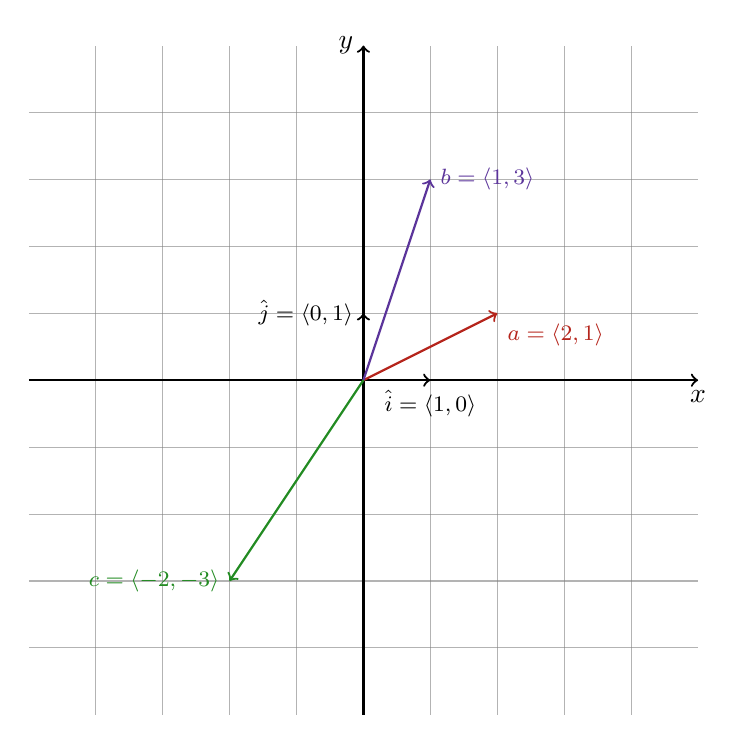
\begin{tikzpicture}[
        vector/.style={->, thick},
        scale=0.85
    ]

    \foreach \i in {-4, -3, ..., 4} {
        \draw[gray, thin, opacity=0.6] (\i, -5) -- (\i, 5);
        \draw[gray, thin, opacity=0.6] (-5, \i) -- (5, \i);
    }
    \draw[vector, black] (-5, 0) -- (5, 0) node[below] {$x$};
    \draw[vector, black] (0, -5) -- (0, 5) node[left] {$y$};

    \draw[vector] (0, 0) -- (1, 0) node[below]
        {\footnotesize $\hat{i} = \langle 1, 0 \rangle$};
    \draw[vector] (0, 0) -- (0, 1) node[left]
        {\footnotesize $\hat{j} = \langle 0, 1 \rangle$};

    \draw[vector, BrickRed] (0, 0) -- (2, 1)
        node[below right, BrickRed]
            {\footnotesize $a = \langle 2, 1 \rangle$};
    \draw[vector, RoyalPurple] (0, 0) -- (1, 3)
        node[right, RoyalPurple]
            {\footnotesize $b = \langle 1, 3 \rangle$};
    \draw[vector, ForestGreen] (0, 0) -- (-2, -3)
        node[left, ForestGreen]
            {\footnotesize $c = \langle -2, -3 \rangle$};
\end{tikzpicture}
\end{figure}

From the graph above, there are two vectors $\hat{i}$ and $\hat{j}$.
They are called ``$i$ hat'' and ``$j$ hat'' respectively.

\begin{definition}{}{}
\textbf{Unit Vectors} are vectors with magnitude $1$ that are used to
specify direction.
\end{definition}

Here, $\hat{i}$ and $\hat{j}$ denote the unit vectors, and they are
the standard symbol. If you wondered if unit vectors are used to
construct vectors, you are right! In our examples above, we can
write each vector as the following.
\begin{align*}
    a &= \langle 2, 1 \rangle = 2 \hat{i} + \hat{j} \\
    b &= \langle 1, 3 \rangle = 1 \hat{i} + 3 \hat{j} \\
    c &= \langle -2, -3 \rangle = -2 \hat{i} - 3 \hat{j}
\end{align*}
Now, let's take a look at vector space $\mathbb{R}^3$. There are
two ways of graphing $3$-dimensional space: right-handed system
and left-handed system. However, we will be using right-hand system
throughout the notes.

\begin{figure}[H]
\centering
\tdplotsetmaincoords{80}{100}
\begin{tikzpicture}[
        tdplot_main_coords,
        axis/.style={->, thick},
        vector/.style={->, very thick},
        scale=0.5
    ]

    \foreach \x in {0,1,...,9}
        \foreach \y in {0,1,...,9} {
			\draw[gray,very thin]
                (\x,0,0) -- (\x,9.5,0);
			\draw[gray,very thin] (0,\y,0) -- (9.5,\y,0);
		}
    \foreach \y in {0,1,...,9}
        \foreach \z in {0,1,...,9} {
			\draw[gray,very thin]
                (0,\y,0) -- (0,\y,9.5);
			\draw[gray,very thin] (0,0,\z) -- (0,9.5,\z);
		}
    \foreach \z in {0,1,...,9}
        \foreach \x in {0,1,...,9} {
			\draw[gray,very thin]
                (0,0,\z) -- (9.5,0,\z);
			\draw[gray,very thin] (\x,0,0) -- (\x,0,9.5);
		}

	\draw[axis] (-2,0,0) -- (10,0,0) node[left] {$x$};
	\draw[axis] (0,-1,0) -- (0,10,0) node[right] {$y$};
	\draw[axis] (0,0,-1) -- (0,0,10) node[left] {$z$};

    \draw[vector] (0, 0, 0) -- (1, 0, 0) node[left]
        {\footnotesize $\hat{i} = \langle 1, 0, 0 \rangle$};
    \draw[vector] (0, 0, 0) -- (0, 1, 0) node[right]
        {\footnotesize $\hat{j} = \langle 0, 1, 0 \rangle$};
    \draw[vector] (0, 0, 0) -- (0, 0, 1) node[above]
        {\footnotesize $\hat{k} = \langle 0, 0, 1 \rangle$};

    \draw[vector, BrickRed] (0, 0, 0) -- (1, 2, 4)
        node[above, BrickRed]
            {\footnotesize $a = \langle 1, 2, 4 \rangle$};
    \draw[vector, RoyalPurple] (0, 0, 0) -- (5, 8, 3)
        node[right, RoyalPurple]
            {\footnotesize $b = \langle 5, 8, 3 \rangle$};
\end{tikzpicture}
\end{figure}

Here, $\hat{i}$, $\hat{j}$, and $\hat{k}$ are the unit vectors.
Going back to the definition of vector spaces, we can write the
following equations for $u = \langle x_1, y_1, z_1 \rangle,
v = \langle x_2, y_2, z_2 \rangle \in \mathbb{R}^3$ and $\alpha
\in \mathbb{R}$.
\begin{align*}
    u \oplus v
    &= \langle x_1, y_1, z_1 \rangle + \langle x_2, y_2, z_2 \rangle
    = \langle x_1 + x_2, y_1 + y_2, z_1 + z_2 \rangle \\
    \alpha \odot u
    &= \alpha \odot \langle x_1, y_1, z_1 \rangle
    = \langle \alpha x_1, \alpha y_1, \alpha z_1 \rangle
\end{align*}
Now that we saw some geometrical interpretation of vector spaces,
let's discuss more information with some problems.

\end{document}


